For this analysis, we first assigned three in-house annotators the task of assigning class labels to each object segmentation in our dataset. The annotators were given the original image (for reference) and the object segmentation and asked to assign a single category to the segment out of $7$ possible categories: animal, building, device, furniture, nature, person, and vehicle. We choose these high-level categories such that a wide range of object classes could be covered under these categories. For example, “device” included object segments such as  utensils, bottles, televisions, computers etc, “nature” included segments like trees, mountains, flowers, and “vehicle” contained segments like cars, bikes, buses, airplanes etc.

Figure \ref{fig:avgMem} shows the distribution of the memorability scores for all $7$ object classes in our dataset. This visualisation gives a sense of how the memorability changes across different object categories. Animal, person, and vehicle are all highly memorable classes each associated with  an average memorability score greater than or close to $0.5$. Interestingly, all other object categories have an average memorability score lower than $0.25$, indicating that humans do not remember objects from these categories very well. In particular, furniture is the least memorable object class with an average memorability score of only $0.14$. This could be possibly due to the fact that most objects from classes like furniture, nature, and building either appear mostly in the background or are occluded which likely decreases their memorability significantly. By contrast, objects from the animal, person, and vehicle classes appear mostly in the foreground, leading to a higher memorability score on average. Interestingly, the topmost memorable objects from building, furniture, and nature tend to have an average memorability score in the range of $0.4 - 0.8$, whereas the topmost memorable objects from classes person, animal and vehicle have an average memorability higher than $0.90$. This is particularly interesting as these top objects are not occluded and most of them tend to appear in the foreground. While the differences in the memorability of different classes could be driven primarily due to factors like occlusion, size, background/foreground, or photographic bias, the distribution in figure \ref{fig:avgMem} suggests that humans remember some object classes such as person, animal, and vehicle irrespective of external nuisance factors and these object classes are \textit{intrinsically} more memorable than others.

\begin{figure*}[t]
\centering
\subfigure{\centering 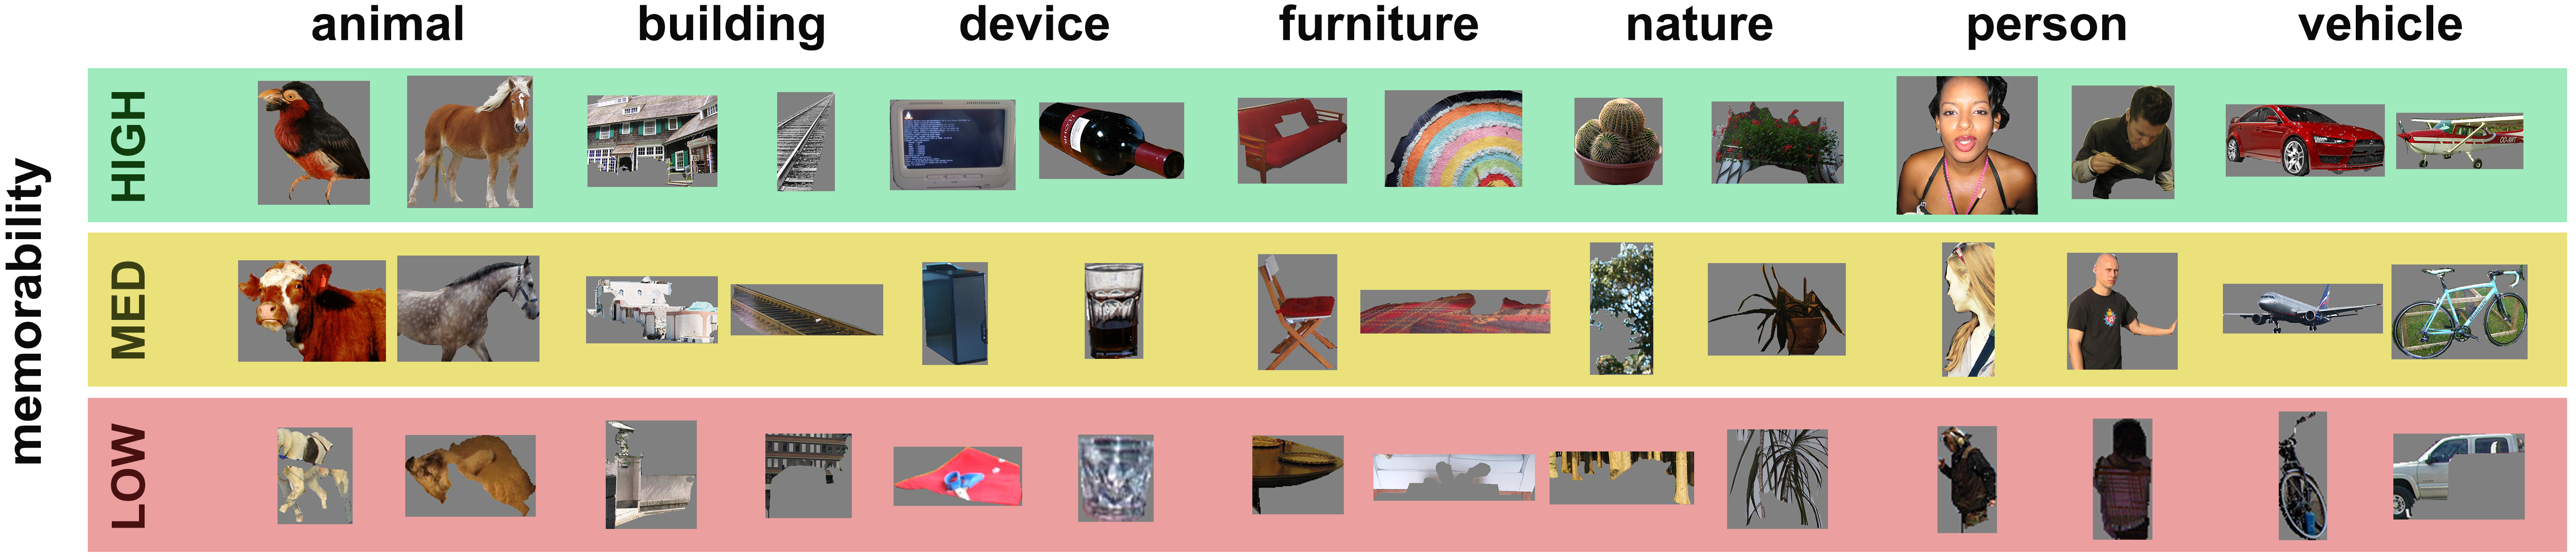
\includegraphics[width=1\textwidth]{figures/results/obLabel/qual_cat.png}}
\vspace{-5mm}\caption{\footnotesize\textbf{Qualitative results from object categories.} add-in later. }\label{fig:obLabelQual}
\end{figure*}

%distribution of the most memorable objects within each class suggest that memorability could be an intrinsic property of an object class.  The right side of the figure presents an interesting analysis This analysis is particularly interesting as these top objects are not occluded and most of them tend to appear in the foreground. The top $20$ most memorable objects from person, animal and vehicle have memorability higher than $0.90$ whereas the average memorability of the top $20$ objects from building, furniture, and nature is lesser than $0.70$. While the differences in the memorability of different classes could be driven primarily due to factors like occlusion, size, background/foreground, the results in table \ref{tab:avgMem} suggest that memorability could be an intrinsic property of an object class and some object classes like person, animal, vehicle are in general intrinsically more memorable than classes like furniture, nature etc.
%
\begin{figure}[t]
\centering
\subfigure{\centering 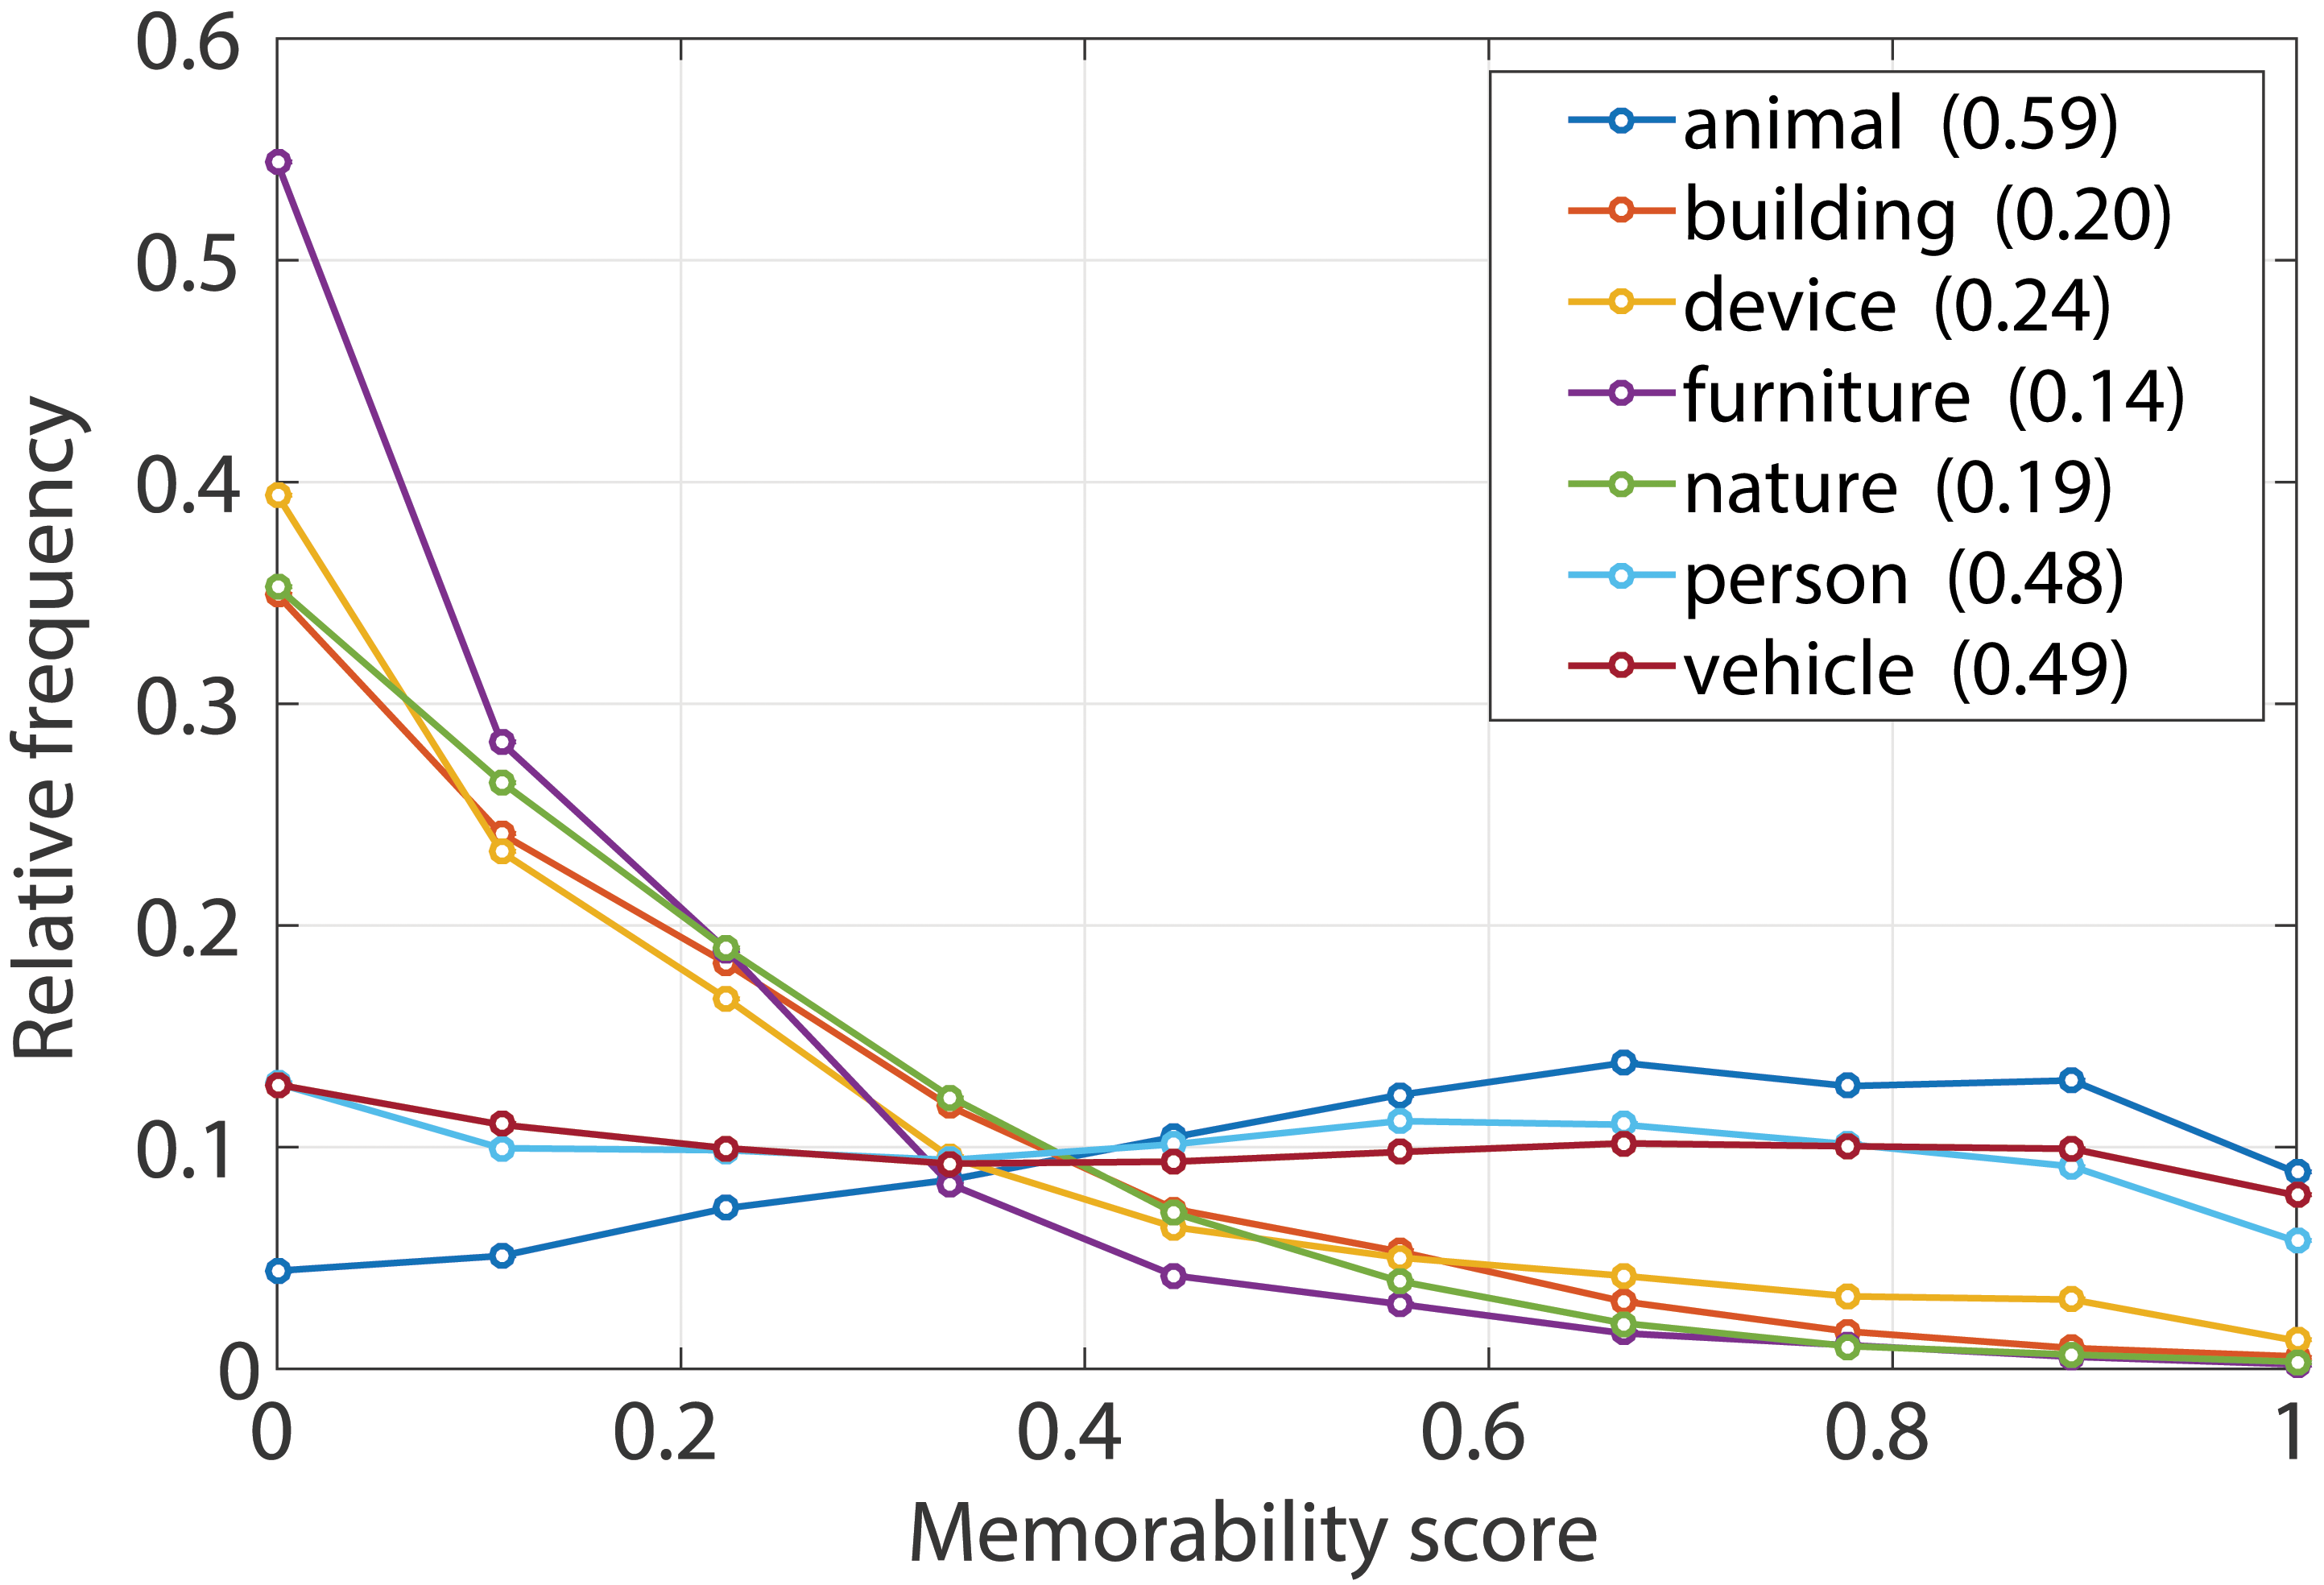
\includegraphics[width=0.45\textwidth]{figures/results/obLabel/memScore_dist2.png}}
\vspace{-5mm}\caption{\footnotesize\textbf{Average memorability per object class.} Figure showing some object classes are more memorable than others. }\label{fig:avgMem}
\end{figure}
